\section{Depth \& breadth tradeoff}

\begin{frame}
	\frametitle{Depth \& breadth tradeoff}
	\begin{itemize}
		\item Shallow architectures are less efficient than deep architectures (in terms of components and parameters)
		\item Derived from formal analysis of boolean circuits \cite{Hastad87}
		\item Space (breadth) can be exchanged for time (depth)
	\end{itemize}
	
	\begin{example}
		\begin{itemize}
			\item Problem: Adding $2$ $N$-bit binary numbers
			\item Intuitive solution: Propagation of carry bit $O(N)$
			\item Shallow solution: DNF $O(2^N)$
		\end{itemize}
	\end{example}
\end{frame}

\begin{frame}
	\frametitle{Example: $N$-bit boolean parity function}
	\begin{itemize}
		\item Problem: Calculate parity of $N$-bit value
	\end{itemize}
	\begin{columns}
		\begin{column}{5cm}
			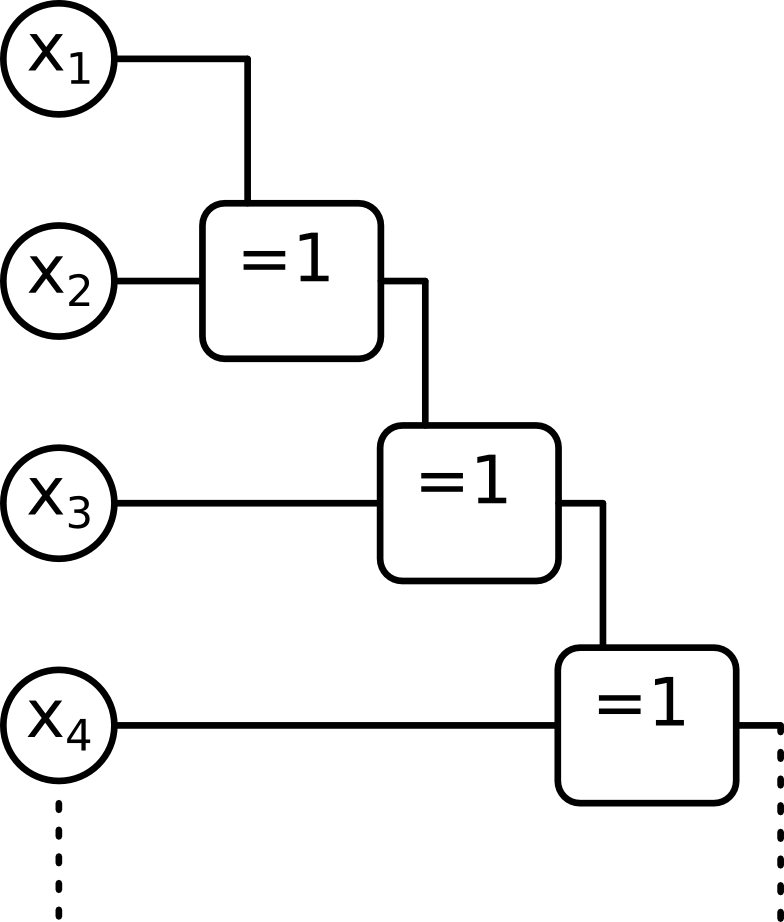
\includegraphics[height=4cm]{images/daisyChainXOR.png}
			\begin{itemize}
				\item Complexity: $O(N)$
			\end{itemize}
		\end{column}
		\begin{column}{5cm}
			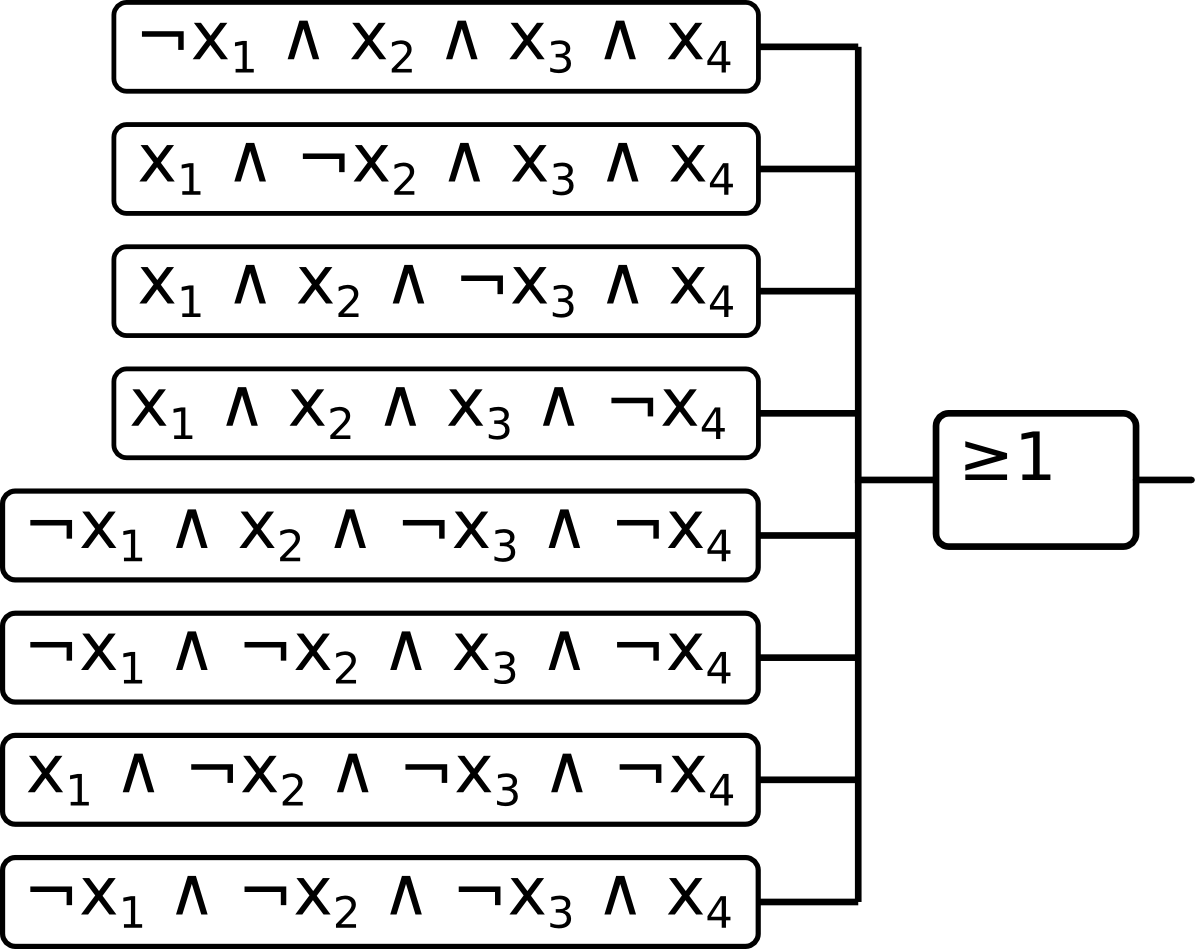
\includegraphics[height=4cm]{images/parityDNF.png}
			\begin{itemize}
				\item Complexity: $O(2^N)$
			\end{itemize}
		\end{column}
	\end{columns}
\end{frame}

\begin{frame}
	\frametitle{General result}
	\begin{Theorem}
		There are polynomial-size logic gate circuits of depth $k$ that require exponential size when restricted to depth $k-1$. \cite{Hastad87}
	\end{Theorem}
	\begin{itemize}
		\item Functions compactly representable by deep architectures have exponential size with a shallow architecture
		\item Components can be shared in deep architectures
		\item Exponential number of components $\Rightarrow$ Bad computational efficiency
		\item Exponential number of training samples required to learn and tune components $\Rightarrow$ Bad statistical efficiency
	\end{itemize}
\end{frame}
